\chapter{Ondorioak.}


\section*{Sarrera}

Gure helburua, eguzki-sistemaren doitasun altuko eta epe luzeko integraziorako, Gaussen metodo inplizituen inplementazio eraginkorra lortzea da. Helburua lortu ote den ala ez galderari erantzuteko, balorazioa bi ikuspegietatik egin behar dela iruditzen zaigu. Batetik, lortutako inplementazioaren aldeko argumentuak azalduz, eraginkorra dela defenditu daiteke. Bestetik, tesian aurkeztutako ikerketa aurretiko lana da eta beraz, garrantzitsua da ere, inplementazioaren eraginkortasuna etorkizunean izan ditzakeen hobekuntzen arabera neurtzea. 

Gakoetako bat, integratu nahi den eguzki-sistemaren ereduaren konplexutasuna da. Eguzki-sistemaren ezagutza gero eta zehatzagoa denez \cite{Kaplan2015}, eredu gero eta konplexuagoak integratu nahi izango direla suposatu daiteke. Zentzu honetan, integrazio metodoa problema konplexuen integraziorako eraginkorra izan beharko luke. Edozein kasutan, argi dago, integrazio metodoak  ez duela aplikatu nahi den problemaren formulazio matematikoa mugatu behar eta askatasun osoa eduki behar dela, ekuazioetan nahi diren efektuak gehitzeko.   

Algoritmo baten eraginkortasuna, konputagailu hardware ingurune bati lotuta dago eta urteekin alda daiteke. Hau da,  konputagailu hardware jakin batean eraginkorra den algoritmoa, hardware berriagotan zaharkitua gera daiteke.  Ezaguna da, egungo konputagailuen ahalmena, konputazio paraleloan oinarritzen dela eta horregatik, idei berritzaileak aplikatu behar direla, algoritmo eraginkorrak garatzeko. Gauss metodo inplizituak, inplementazio aukera asko eskaintzen dituenez, zenbakizko integrazioen arloan idei berriak garatzeko metodo egokiak direla \cite{Dongarra2017} esaten ausartuko ginateke.   


\section*{Eguzki-sistemaren integraziorako inplementazioa.}


Eguzki-sistemaren integraziorako, Runge-Kutta metodo inplizitu orokorra (IRK) aplikatu dugula azpimarratu behar dugu. Hori dela-eta, inplementazioa sinplea da eta inplementazioak, metodoaren ezaugarri on guztiak heredatzen ditu. Azken finean, puntu-finkoaren iterazioan oinarritutako IRK inplementazio estandarra aplikatu dugu, formulazio eta geratze irizpide bereziekin. Epe luzeko integrazioetarako, metodoa sinplektikoa izatea garrantzitsua da. Baina, IRK metodoaren formulazio estandarrak  sinplektikotasuna ez duenez ziurtatzen, IRK metodoa aplikatzeko formulazio berria proposatu dugu. Bestalde, inplementazio estandarraren geratze irizpidea hobetu dugu. Laburtuz, IRK inplementazio estandarrean oinarritzerakoan, inplementazio berri batek izan ditzakeen konplexutasunak ekidin ditugu. 

Kepler-en fluxuan oinarritutako aldagai aldaketa, ebatzi nahi dugun problemari lotuta dago. Aldagai aldaketa hau, teknika orokor baten aplikazioa da; hau da, ekuazio diferentzialetatik zati bat desagerrarazteko helburuarekin definitutako aldagai aldaketa aplikatzearena. Aldagai aldaketa honekin, ekuazio diferentzialetatik alde Kepleriarrari dagokion zatia desagertzen da eta mantso aldatzen diren ekuazio diferentzialak lortzen ditugu.  Aldagai berriekiko ekuazio diferentzialek, hiru abantaila dituzte. Lehenik, eguzki-sistemaren trunkatze errore nagusiena ezabatu dugunez, integrazioan urrats luzera handiagoak erabil daitezke. Bigarrenik, integrazioaren urratsaren konputazioaren baturan,
\begin{equation*}
% (\tilde{y}_{n+1}, e_{n+1}) \leftarrow \text{batura konpensatua}(\tilde{y}_n, e_n,\delta_n),
 y_{n+1}=y_{n}+\delta_n,
\end{equation*}
$\delta_n$ gehikuntzak magnitude txikia du eta beraz, batuketa honetan informazio gutxiago galduko da. Gainera, $\delta_n$ doitasun altuan kalkulatzeak, abantaila areagotu egiten du. Hirugarrenik, puntu-finkoaren konbergentzia azkarra izango da.

Eguzki-sistema eredu konplexuetan, Kleperiarrak ez diren indarrak aplika daitezke. Aldagai hauen konbergentzia azkartzeko, Newton sinplifikatuaren iterazioan oinarritutako inplementazioa aplikatzea komeniko da.                  

Gauss metodoa, neurri batean  splitting eta konposizio metodoen antzekoak dira. 
\begin{align*}
\text{Konposizio metodoa} \ \ &\equiv \ \ \text{Gauss metodoa, aldagai aldaketa gabe}.\\
\text{Splitting metodoa}  \ \ &\equiv \ \  \text{Gauss metodoa, aldagai aldaketarekin}.
\end{align*}

Splitting metodoekiko antzekotasuna azaltzeko, (\ref{eq:stverlet})~\emph{Störmer-Verlet} splitting metodoarekin konparatuko dugu. \emph{Störmer-Verlet} metodoa, era honetan aplikatzen da:  fluxua $h/2$ aurreratu, perturbazioak kalkulatu eta berriz,  fluxua $h/2$ aurreratu. Kepler-en fluxuan oinarritutako aldagai aldaketa aplikatzen dugunean, gauza bera egiten ari gara:  fluxua $h/2$ aurreratu, perturbazioak kalkulatu (aldagai berrietan eta beraz, hobeto kalkulatzen dugu),  fluxua $h/2$ aurreratu (\ref{fig:urratsBat}~irudia).

\begin{figure} [h!]
{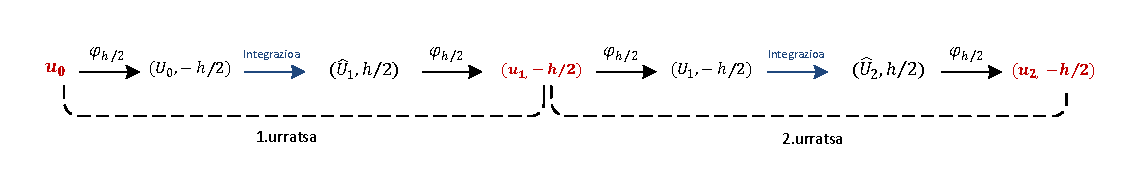
\includegraphics [width=16cm, height=4cm] {urratsBat}}
\caption{\small Gauss metodoan, Kepler-en fluxuan oinarritutako aldagai aldaketa aplikatzen dugunean, urratsaren konputazioa}
\label{fig:urratsBat}
\end{figure} 

Splitting metodoak oso eraginkorrak dira eta eguzki-sistemaren eredu sinplearen integrazioen  esperimentuek, hori erakutsi digute. Baina eredu errealistagoak (gorputz kopurua handitzen delako edota erlatibitate efektua kontutan hartzen delako) integratzeko, Kepler fluxuan oinarritutako Gauss metodoak, splitting metodoekiko abantailak hauek izango dituela azpimarratuko dugu:  

\begin{enumerate}

\item Ordena altuko metodoak.

Konposizio eta  splitting metodo optimoenak, $p=10$ ordenakoak dira. Gauss metodoei dagokienez, edozein ordenako metodoak eraiki daitezke. Doitasun bikoitzeko konputazioetarako, $s=6$ ataletako metodoa eraginkorrena kontsideratzen da \cite{Hairer2008} baina doitasun altuagoko konputazioetarako, ordena altuagoko metodoak aplikatzea gomendagarria da.
Adibidez, Gaussen $s=16$ ataletako metodoa ($p=32$ ordenakoa) era honetan aplika daiteke: $80$-biteko doitasuneko  (\emph{long double}) integrazioa kalkulatu, eta inplementazioaren zati batzuk $128$-biteko doitasunean, konputatu soluzioaren doitasuna hobetzeko.  

\item Paralelizagarria.

Gauss metodoaren $s$-ataletako funtzioen ebaluazioak independenteak dira eta modu paraleloan exekutatu daitezke. Eguzki-sistemaren eredu konplexuagoa kontutan hartzen den neurrian, paralelizazioak abantaila handiagoa suposatuko du. Gauss metodoaren paralelizazio gaitasun hau azpimarratzekoa da, egungo algoritmo azkarren diseinua, kodearen paralelizazioan oinarritzen baita.

\item Hamiltondar orokorrak.

Gauss metodoa, edozein sistema Hamiltondarrari aplika dakioke. Splitting metodoa, ordea, sistema Hamiltondar banagarrietan bakarrik aplika daitezke; eguzki-sistemaren eredu errealistak integratzeko, Hamiltondarraren egitura mantendu behar da eta hainbat indar ez grabitazionalak  gehitzeko, zailtasunak izan ditzakegu. 

\item Malgutasuna.

Splitting metodoen konputazioak, modu trinkoan kalkulatu behar dira, hau da, atalen konputazioak sekuentzialki exekutatzen dira eta konputazioak ez ditu aldaerak onartzen. Gauss metodoaren ekuazio inplizituak ebazteko, ordea, teknika ezberdinak konbina daitezke eta eraginkortasuna hobetzeko aukera asko eskaintzen dizkigu. Adibidez, iterazio gehienak problemaren eredu sinple batekin, doitasun baxuan kalkula daitezke  \cite{Beylkin2014} eta bukaerako iterazio pare bat eredu osoarekin, doitasun altuan. 

\item Birparametrizazioa.

Birparametrizazio, eguzki-sistemaren integrazioetarako tresna baliagarria dela frogatu da \cite{Fukushima2007,Rauch1998} eta Gauss metodoan,  teknika hau zuzenean aplika daiteke. Splitting metodoetan, ordea, birparametrizazioa ezin daiteke erabili eta integrazioetan zailtasunak agertzen direnean (esaterako, planeta baten eszentrikotasuna handitzen denean), orduan integrazioaren tarte batean urratsaren luzera txikitu behar dute soluzioaren doitasuna mantentzeko \cite{Laskar2009}.

\end{enumerate}


\section*{Etorkizuneko lanak.}


Eguzki-sistemaren integraziorako inplementazioa garatzeko aukerak zehaztuko ditugu. Lehen eginbeharra, eguzki-sistemaren eredu konplexuagoak integratzea da eta zehazki, arlo honetan  aplikatzen den eguzki-sistemaren ereduekin \cite{Laskar2011} gure inplementazioaren jokabidea aztertzea. Eredu sinplearekin lortutako emaitzekin baikorrak izateko arrazoiak baditugu eta eredu konplexuagoekin, gure inplementazioaren abantaila areagotu daitekeela pentsatzen dugu. inplementazioaren eraginkortasuna hobetzeko tresna nagusienak hauek izan daitezke:


\begin{enumerate}
\item Eredu deskonposaketan oinarritutako teknikak.

Inplementazioa eraginkorragoa egiteko, lehen iterazioak eredu sinpleagoarekin kalkula daitezke eta bukaerako iterazioak, eredu konplexuagoarekin.

\item Denbora birparametrizazioak.

Gorputzen gerturatzeen tratamendurako, denbora birparametrizazio teknikak aplikatzea. 

\item Problema oszilakorren teknikak.

Problema oszilakorren tratamendu aljebraikoan oinarritutako hobekuntza teknikak (metodo prozesatuak, promediatuen teknikak).
Wisdom-ek \cite{Wisdom2006} bere integrazio metodoen doitasuna hobetzeko teknikekin (\emph{symplectic correctors}) erlazionatutakoak dira.

\item Paralelizazio eta bektorizazio teknika aurreratuak.



\end{enumerate} 








